\chapter{Conceptual Design}

\section{Requirements Analysis}



\section{Reorganize sentences for specific concepts}


\begin{tcolorbox}[title=General Phrases]
We want to create a database that manages decentralized logistics operations through several operational centers, storing information about orders, teams, and customers. The company offers customized warehouse management services, including long-term storage and expedited shipping.
\end{tcolorbox}

\begin{tcolorbox}[title=Phrases related to Operational Centers]
Operational centers are distributed across regions, each responsible for handling local storage and shipments.  

For each operational center, we will hold name, address, city/province, and number of employees.  

Operational centers have management teams.
\end{tcolorbox}

\begin{tcolorbox}[title=Phrases related to Orders]
Orders can be placed by customers via phone, email, or online.  

For each order, we will hold type, date, cost, and customer information.  

Every order is associated with a single business account.  

Orders can be of three types: regular, urgent, or bulk (large quantities).
\end{tcolorbox}

\begin{tcolorbox}[title=Phrases related to Business Accounts]
Each business account will be identified by a unique code.  

Each customer may have one or more business accounts.  

Every order is associated with a single business account.
\end{tcolorbox}

\begin{tcolorbox}[title=Phrases related to Teams]
For each team, we will identify them via a unique code, and we will hold name and number of orders handled.  

Teams consist of employees, and the number of employees may vary depending on the required workload.  

The company maintains a performance evaluation system that assigns a score to each team based on delivery times and customer feedback.
\end{tcolorbox}

\begin{tcolorbox}[title=Phrases related to Customers]
Each customer may have one or more business accounts.  

Customers can be classified as individual or business, each identified by a unique alphanumeric code, with contact details and order history.
\end{tcolorbox}

\begin{tcolorbox}[title=Phrases related to Employees]
Teams consist of employees, and the number of employees may vary depending on the required workload.
\end{tcolorbox}

\section{Level of abstraction}
For \textbf{customer information}, we consider \textit{name}, \textit{surname}, and \textit{date of birth} for individual customers, and \textit{company name} and \textit{address} for business customers, where the address consists of \textit{street}, \textit{civic number}, \textit{city}, \textit{province}, \textit{region}, and \textit{state}.  

For \textbf{contact details}, we consider \textit{phone number} and \textit{email}.  

\textbf{Specialized personnel} is replaced by \textit{employees}.  

\textbf{Number of members} is replaced by \textit{number of employees}.  

\textbf{Number of operations} is replaced by \textit{number of orders}.

\section{Glossary of terms}
\begin{table}[h!]
    \resizebox{\textwidth}{!}{
    \begin{tabular}{|c|p{5cm}|p{3cm}|p{3cm}|}
    \hline
    \textbf{Term} & \textbf{Description} & \textbf{Synonyms} & \textbf{Connections} \\
    \hline
    Operational Center & Decentralized locations handling local storage and shipments. Characterized by name, address, city/province, and number of employees. & / & Team \\
    \hline
    Order & Requests for services or goods from customers, identified by type (regular, urgent, or bulk). Includes type, date, cost, and customer details. & Operation & Customer, Business Account, Team \\
    \hline
    Business Account & Accounts tied to customers, containing unique codes and details like orders and customer type (individual or business). & Account & Customer, Order \\
    \hline
    Team & Groups of employees linked to an operational center, evaluated on delivery times and customer feedback. & Management Team & Operational Center, Order, Employee \\
    \hline
    Customer & Individuals or businesses placing orders. Identified by unique alphanumeric codes, contact details, and order history. & Individual, Business & Order, Business Account \\
    \hline
    Employee & Specialized personnel working in teams and handling orders. & Specialized Personnel & Team \\
    \hline
    \end{tabular}
    }
    \end{table}

\subsection{Skeleton ER Schema}
\begin{figure}[H]
    \centering
    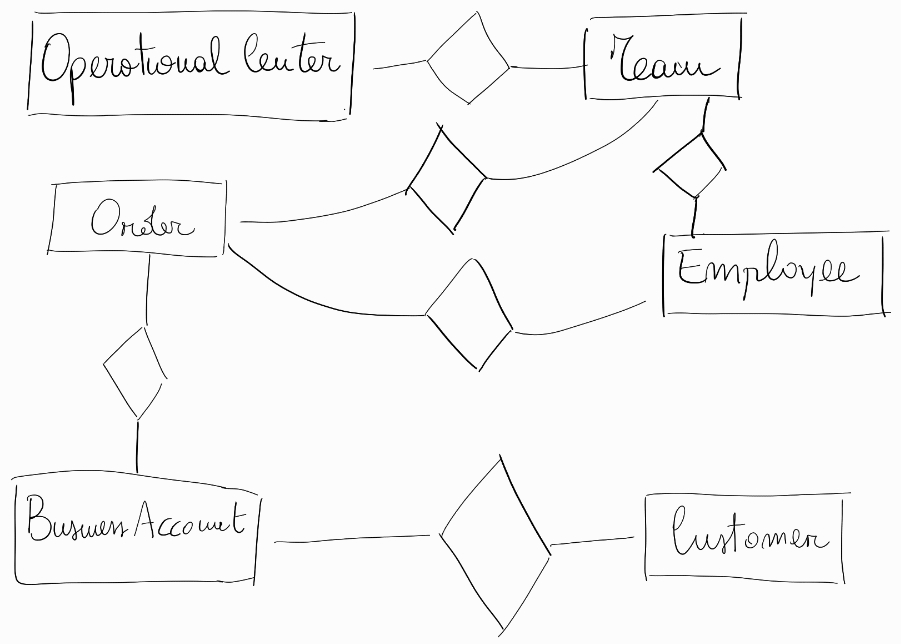
\includegraphics[width=0.8\textwidth]{img/skeleton.png}
\end{figure}

\subsection{Final ER Schema}
\begin{figure}[H]
    \centering
    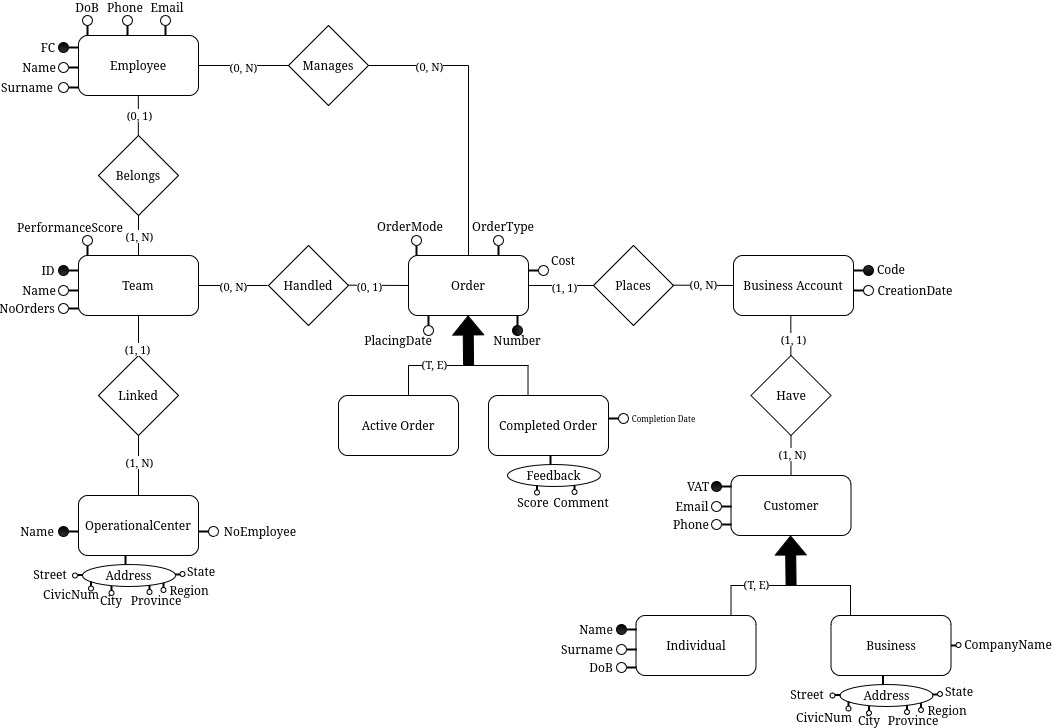
\includegraphics[width=0.8\textwidth]{img/ER.jpg}
\end{figure}

\begin{itemize}[label=-]
    \item There are three redundancies: \texttt{NoOrders} and \texttt{PerformanceScore} in \texttt{Team} and \texttt{NoEmployee} in \texttt{Operational Center}, that will be evaluated later.
    \item There are two generalizations for \texttt{Order} and \texttt{Customer}, that will be evaluated later.
\end{itemize}

\section{Business Rules}
\begin{itemize}
    \item Employees linked to an order must be in the same team that handle the order.
    \item Number of employees is the sum of all employees in a team.
    \item Number of orders is the sum of all orders handled by a team.
    \item Completion date cannot be before placing date.
    \item PerformanceScore is computed as the mean of all feedbacks.
    \item A team has a maximum of 8 members.
    \item OrderType must be of three types: regular, urgent, or bulk.
    \item OrderMode must be of three types: phone, email, or online.
    \item Feedback of CompletedOrder must be between 1 and 5.
    \item A feedback cannot be given before the order is completed.
    \item A team must be assigned before an order is completed.
    \item A team cannot be changed after an order is completed.
    \item Employees of a completed order cannot be changed.
    \item An order can be deleted only if there are not information for the business account or for the feedback computation.
\end{itemize}

